\chapter{Sistema/Modelo/Método}

\section{Modelo}
El cubo de Rubik original $3 \times 3 \times 3$ esta compuesto de 3 tipos de piezas distintas:
\begin{itemize}
	\item \textbf{centros}: piezas con un sólo color, que sólo rotan sobre su eje, 6 en total.
	\item \textbf{aristas}: piezas con 2 colores, 12 en total.
	\item \textbf{esquinas}: piezas con 3 colores, 8 en total.
\end{itemize}
La cantidad total de stickers (también llamados \textit{facelets}) es entonces 54.
\begin{figure}[h!]
	\centering
	\subcaptionbox{Centros}{%
		\includegraphics[width=0.30\textwidth]{figures/centers}
	}%
	\hfill
	\subcaptionbox{Aristas}{%
		\includegraphics[width=0.30\textwidth]{figures/edges}
	}%
	\hfill
	\subcaptionbox{Esquinas}{%
		\includegraphics[width=0.30\textwidth]{figures/corners}
	}%
	\caption{Los 3 tipos de piezas del cubo de Rubik.}
\end{figure}

\subsection*{Convenciones}
Existe una notación estándar para describir los ejes, las caras y los facelets del cubo.
Los 3 ejes de coordenadas del sistema de referencia utilizado se definen de la siguiente manera:
\begin{itemize}
	\item $x$: eje que atraviesa las caras derecha e izquierda del cubo, con respecto al observador.
	\item $y$: eje que atraviesa las caras superior e inferior del cubo.
	\item $z$: eje que atraviesa las caras frontal y trasera del cubo.
\end{itemize}
Así, cada una de las piezas esquina del cubo tiene 1 color por eje.

Las caras del cubo se identifican mediante la letra inicial de la palabra en inglés que identifica su posición con respecto al observador.
Éstas letras son \textit{U} (up), \textit{R} (right), \textit{F} (front), \textit{D} (down), \textit{L} (left) y \textit{B} (bottom).

\begin{figure}[h!]
	\centering
	\subcaptionbox{Ejes}{%
		\includegraphics[width=0.45\textwidth]{figures/axes}
	}%
	\hfill
	\subcaptionbox{Caras}{%
		\includegraphics[width=0.45\textwidth]{figures/faces}
	}%
	\caption{Notación de ejes y caras del cubo.}
\end{figure}
De manera similar, los movimientos posibles de cada cara del cubo también quedan descritos por la letra correspondiente de la cara rotada.
En este punto, se decidió adoptar una notación ligeramente diferente de la estandar.
\textit{XN} indica que la cara \textit{X} rota en $90 \times N$ grados, donde los grados se miden utilizando la regla de la mano derecha sobre un vector normal a la superficie de la cara a rotar.
Entonces, por ejemplo \textit{R1} significa rotar cara frontal en 90 (o -270) grados, \textit{R2} es rotar cara frontal en 180 (o -180) grados y \textit{R3} rotar cara frontal en 270 (o -90) grados.

\begin{figure}
	\centering
	\includegraphics[scale=0.3]{figures/R1}
	\caption{Flecha azul: movimiento \textit{R1} ($90$ grados sentido horario). Flecha amarilla: movimiento \textit{R3} (90 grados sentido antihorario).}
	\label{moveR}
\end{figure}

Estos ángulos bastan para describir todos los movimientos posibles, ya que 360 equivale a una operación nula y cualquier otro ángulo dejaría el cubo en un estado inválido (bloqueando los movimientos de las demás caras).

Las piezas se identifican con las letras de las caras a las que pertenecen. Por lo tanto las caras son \textit{U}, \textit{R}, \textit{F}, \textit{D}, \textit{L} y \textit{B}, las aristas son \textit{UF}, \textit{UR}, \textit{UL}, \textit{UB}, \textit{DF}, \textit{DR}, \textit{DL}, \textit{DB}, \textit{FR}, \textit{FL}, \textit{BR} y \textit{BL} y las esquinas son \textit{URF}, \textit{URB}, \textit{ULF}, \textit{ULB}, \textit{DRF}, \textit{DRB}, \textit{DLF}, y \textit{DLB}.

El estado final del cubo se representó como arreglo de 54 elementos, donde cada elemento representa un facelet. El orden de los facelets se muestra en la figura~\ref{faceletorder}.
La asignación de colores a cada cara es totalmente arbitraria y no tiene importancia para el sistema desarrollado. Lo importante es que una vez se decida una asignación se mantenga hasta el final.

\tikzset{boxu/.style={draw, minimum width=1cm, minimum height=1cm, fill=red, text=white}}
\tikzset{boxr/.style={draw, minimum width=1cm, minimum height=1cm, fill=blue, text=white}}
\tikzset{boxf/.style={draw, minimum width=1cm, minimum height=1cm, fill=yellow}}
\tikzset{boxd/.style={draw, minimum width=1cm, minimum height=1cm, fill=orange, text=white}}
\tikzset{boxl/.style={draw, minimum width=1cm, minimum height=1cm, fill=red, text=white}}
\tikzset{boxl/.style={draw, minimum width=1cm, minimum height=1cm, fill=green}}
\tikzset{boxb/.style={draw, minimum width=1cm, minimum height=1cm, fill=white}}
\tikzset{boxx/.style={draw, minimum width=1cm, minimum height=1cm, fill=red, text=white}}
\tikzset{boxy/.style={draw, minimum width=1cm, minimum height=1cm, fill=green}}
\tikzset{boxz/.style={draw, minimum width=1cm, minimum height=1cm, fill=blue, text=white}}
\tikzset{boxc/.style={draw, minimum width=1cm, minimum height=1cm}}

\begin{figure}[ht!]
	\centering
	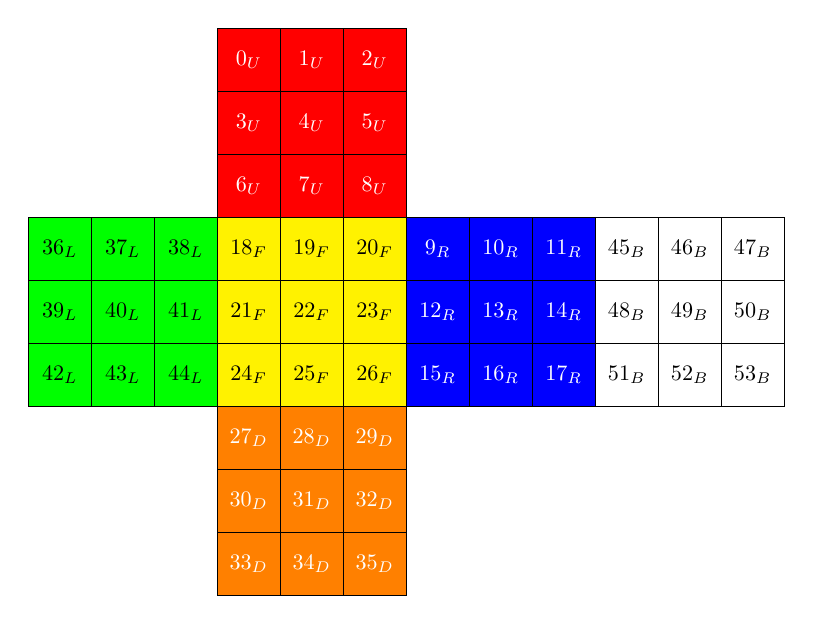
\begin{tikzpicture}[scale=0.8,every node/.style={scale=0.8}]
		\foreach \x in {0,...,2} {
			\foreach \y in {0,...,2} {
			 	\pgfmathsetmacro\result{int(3*\x+\y)}
				\node[boxu] at (3+\y, 8-\x) {$\result_U$};
			}
		}
		\foreach \x in {0,...,2} {
			\foreach \y in {0,...,2} {
				\pgfmathsetmacro\result{int(3*\x+\y + 36)}
				\node[boxl] at (\y, 5-\x) {$\result_L$};
			}
		}
		\foreach \x in {0,...,2} {
			\foreach \y in {0,...,2} {
				\pgfmathsetmacro\result{int(3*\x+\y + 18)}
				\node[boxf] at (\y+3, 5-\x) {$\result_F$};
			}
		}
		\foreach \x in {0,...,2} {
			\foreach \y in {0,...,2} {
				\pgfmathsetmacro\result{int(3*\x+\y + 9)}
				\node[boxr] at (\y+6, 5-\x) {$\result_R$};
			}
		}
		\foreach \x in {0,...,2} {
			\foreach \y in {0,...,2} {
				\pgfmathsetmacro\result{int(3*\x+\y + 45)}
				\node[boxb] at (\y+9, 5-\x) {$\result_B$};
			}
		}
		\foreach \x in {0,...,2} {
			\foreach \y in {0,...,2} {
				\pgfmathsetmacro\result{int(3*\x+\y + 27)}
				\node[boxd] at (\y+3, 2-\x) {$\result_D$};
			}
		}
	\end{tikzpicture}
	\caption{Orden de los facelets. El valor representa su posición el arreglo y el subíndice la cara a la que pertenece.}
	\label{faceletorder}
\end{figure}

\section{Sistema}
El sistema desarrollado consiste de los siguientes módulos:
\begin{description}
	\item[Manipulador:] Módulo que se encarga de mover las articulaciones y grippers del robot.
	\item[Capturador:] Módulo encargado de la visión del robot.
	\item[Extractor:] Módulo encargado de detectar regiones de interés y el color representativo de cada region.
	\item[Clasificador:] Módulo encargado de agrupar colores similares para obtener el estado del cubo como una permutación.
	\item[Resolutor/Solucionador:] Modulo encargado de buscar una secuencia de rotaciones de caras que lleven al cubo a su estado resuelto.
\end{description}

\subsection{Manipulador}
Este módulo se encarga de la parte hardware del sistema, es decir los movimientos de las articulaciones del robot y la apertura, cierre y calibración de los grippers. Para mover los brazos del robot se usa una combinación de cinemáticas inversas y manipulación directa de ángulos de sus articulaciones.



\subsection{Capturador}
Este módulo se encarga de obtener imágenes del cubo. Cada cara es capturada una vez.
\subsection{Extractor}
Este módulo se encarga de encontrar las regiones de interés
\subsection{Clasificador}
\subsection{Solucionador}


El orden de ejecución final es el siguiente:
\begin{enumerate}
	\item Manipulador: Robot recoge el cubo de Rubik con su brazo izquierdo. La posición donde queden ubicados los grippers corresponderán a las caras \textit{R} y \textit{L}.
	\item Manipulador+Capturador: Robot mueve brazo izquierdo de manera de apuntar las caras \textit{F}, \textit{B} y \textit{D} (en ese orden) directamente hacia la cámara ubicaza en su cabeza. Cada cara es fotografiada una vez y se guarda la matriz correspondiente a la imagen RGB y los 9 círculos detectados en cada cara.
	\item Manipulador: Robot pasa el cubo de su mano izquierda a su mano derecha.
	\item Manipulador+Capturador: Robot mueve brazo derecho de manera de apuntar las caras \textit{R}, \textit{L} y \textit{U} (en ese orden) directamente hacia la cámara ubicaza en su cabeza. Cada cara es fotografiada una vez y se guarda la matriz correspondiente a la imagen RGB y los 9 círculos detectados en cada cara.
	\item Extractor: Se extrae el color representativo de cada uno de los 54 círculos, dando a lugar a un arreglo de 54 colores RGB.
	\item Clasificador: Se agrupan los colores del paso anterior para obtener el estado del cubo, como una permutación.
	\item Solucionador: Se toma la permutación obtenida y se entrega una secuencia de rotaciones para resolver el cubo.
	\item Manipulador: Se realizan las rotaciones moviendo los brazos del robot, cambiando de mano cuando sea necesario.
\end{enumerate}
